\documentclass[11pt]{article}

\usepackage{amsmath}
\usepackage{amssymb,latexsym}
\usepackage{amsthm}
\usepackage[spanish]{babel}
\usepackage[pdftex]{graphicx} % PDFLaTeX
\DeclareGraphicsExtensions{.png,.pdf,.jpg}
\usepackage{epsf}
\usepackage{graphicx}

\newtheorem{teorema}{Teorema}[section]
\newtheorem{lema}[teorema]{Lema}
\theoremstyle{definition}
\newtheorem{definicion}[teorema]{Definici\'on}
\newtheorem{problema}{Problema}
\newtheorem{ejemplo}{Ejemplo}

\renewcommand{\baselinestretch}{1.2}
\usepackage[bottom]{footmisc}  % places footnotes at page bottom
\usepackage[latin1]{inputenc}      %    tipo de codificacion del documento: applemac,

\usepackage{subfigure}
\spanishdecimal{.}
\usepackage{amssymb,amsmath,latexsym,amsfonts}
\usepackage{rotating}
\usepackage{indentfirst}        


\begin{document}

\title{C�LCULO PARA EL AN�LISIS ECON�MICO}
\author{\textbf{ESCUELA SUPERIOR DE ECONOM�A}}
\date{\large{M\'exico, D.F., 27 de Agosto de 2010}}
\def\contentsname{Contenido}

\newpage

\setcounter{page}{1}

\section{Derivadas}
\newpage

\setcounter{page}{1}

\section{Optimizaci�n libre con una variable}
\subsection{M\'aximos y m\'{\i}nimos relativos y absolutos}
\textbf{Introducci\'on}
\medskip

En esta secci\'on resolveremos problemas que impliquen maximizar o
mi\-ni\-mi\-zar una cantidad. Por ejemplo, podr\'{\i}amos tener que
maximizar una ganancia o minimizar un costo. La parte crucial
consiste en expresar la cantidad que se debe maximizar o minimizar
como funci\'on  de alguna va\-ria\-ble contenida en el problema.
Luego diferenciamos y probamos los valores cr\'{\i}ticos
resultantes. Para esto pueden usarse las pruebas de la primera o de
la segunda derivada, aunque puede ser obvio por la naturaleza  si un
valor cr\'{\i}tico representa o no una respuesta apropiada. Como
nuestro inter\'es estriba en los m\'aximos y m\'{\i}nimos absolutos,
a veces tendremos que examinar los puntos extremos del dominio de la
funci\'on.

\subsubsection{M�todo anal�tico}

\begin{definicion}
Una funci\'on $f$ tiene un \textbf{m\'aximo absoluto} en $x = x_0$,
si $f(x_0) \geq f(x)$ para toda $x$ en el dominio de $f$. El m\'aximo
absoluto es $f(x_0)$. Una funci\'on $f$ tiene un \textbf{m\'{\i}nimo absoluto}
en $x = x_0$, si $f(x_0) \leq f(x)$, para toda $x$ en el dominio de $f$.
El m\'{\i}nimo absoluto es $f(x_0)$.
\end{definicion}

Los valores  m\'aximo y m\'{\i}nimo absoluto se llaman
\textbf{extremos absolutos}. Los extremos absolutos tambi\'en
suelen denominarse extremos \textbf{ globales}, para distinguirlos
de los extremos locales, que se definen a continuaci\'on.


\begin{definicion}
Una funci\'on $f$ tiene un \textbf{m\'aximo relativo} en $x = x_0$,
si existe un intervalo abierto que contenga a $x_0$, sobre el cual
$f(x_0) \geq f(x)$ para toda $x$ en el intervalo. El m\'aximo
relativo es $f(x_0)$. Una funci\'on tiene un \textbf{m\'{\i}nimo
relativo} en $x = x_0$, si existe un intervalo abierto que contenga
a $x_0$, sobre el cual $f(x_0) \leq f(x)$, para toda $x$ en el
intervalo. El m\'{\i}nimo relativo es $f(x_0)$.
\end{definicion}

Cuando aludamos a un m\'aximo o un m\'{\i}nimo relativo lo llamaremos a cada uno extremo relativo.

\begin{definicion}
Si $x_0$ est\'a en el dominio de $f$ y $\frac{df}{dx} (x_0) = 0$ o $\frac{df}{dx} (x_0)$
no est\'a definida, entonces $x_0$ se denomina valor cr\'{\i}tico de $f$. Si $x_0$ es un
\textbf{valor cr\'{\i}tico} de $f$, entonces el punto $(x_0, f(x_0)$ se le llama \textbf{punto cr\'{\i}tico}.
\end{definicion}

\subsection{Criterios de la primera y segunda derivada }

\textbf{Criterio de la derivada para hallar M\'aximos y
M\'{\i}nimos:}
\begin{enumerate}
  \item[] \textbf{1er paso.} Calcular $\frac{df}{dx}(x)$.
  \item[]\textbf{2o. paso.}   Determinar los valores de $x$ en que $\frac{df}{dx} (x) = 0 $ o no est\'a definida
  (estos valores incluyen valores cr\'{\i}ticos y puntos de discontinuidad).
  \item[]\textbf{3er. paso.} Calcular $\frac{d^2 f}{dx^{2}} (x)$.
  \item[] \textbf{4o. paso.}
  Evaluar $\frac{d^2 f}{dx^{2}} (x_0)$ para cada valor cr\'{\i}tico
  $x_0$. Entonces
  \begin{enumerate}
  \item[i)] Si $\frac{d^2 f}{d x^{2}} (x_0) < 0$, entonces $f$ tiene un m\'aximo reativo en $x_0$.
  \item[ii)] Si $\frac{d^2 f}{d x^{2}} (x_0) > 0$, entonces  $f$ tiene un m\'{\i}nimo relativo en $x_0$.
  \item[iii)] Si $\frac{d^2 f}{d x^{2}} (x_0) = 0 $, entonces el criterio no es concluyente.
  \end{enumerate}
\end{enumerate}

\begin{definicion}
Una funci\'on $f$ tiene un \textbf{punto de inflexi\'on} cuando $x =
x_0$, si y s\'olo si $f$ es continua en $x_0$, y $f$ cambia de
concavidad en $x_0$.
\end{definicion}

\begin{ejemplo}
Encontar los valores m\'aximo y m\'{\i}nimo absolutos de $f(x)= x^3+3x^2 -2$ en $[-3,1]$

\textbf{Soluci\'on:}
\medskip

\begin{enumerate}
  \item[] \textbf{1er paso.} Calculemos $\frac{df}{dx}(x)$.
  \[
 \frac{df}{dx} = 3x^2  + 6x
  \]
  \item[]\textbf{2o. paso.}   Determinemos los valores de $x$ en que $\frac{df}{dx} (x) = 0 $
 \begin{align*}
    \frac{df}{dx} &= 0 \\
    3x^2  + 6x   & = 0 \\
    3x(x  +  2) & =0
 \end{align*}
 Resolviendo las ecuaciones $3x = 0$ y $x + 2 = 0$, tenemos que los valores cr\'{\i}ticos son  $x_1 =
 0$ y $x_2 = -2$.

  \item[]\textbf{3er. paso.} Hallemos la segunda derivada
\[
 \frac{d^2 f}{dx^{2}} (x) =  6x + 6.
\]

  \item[] \textbf{4o. paso.}
  Evaluemos  $\frac{d^2 f}{dx^{2}} (x)$ en cada  valor cr\'{\i}tico.
  Entonces
\begin{align*}
\frac{d^2 f}{dx^{2}} (0) &= 6(0) + 6 \\
\frac{d^2 f}{dx^{2}} (0) &= 6
\end{align*}
Por lo que $x_1 =0$ es la abscisa de un m\'{\i}nimo.
\begin{align*}
\frac{d^2 f}{dx^{2}} (-2) &= 6(-2) + 6 \\
\frac{d^2 f}{dx^{2}} (-2) &= -6
\end{align*}
En consecuencia el punto $x_2 = -2$ es la abscisa de un m\'aximo.
\end{enumerate}

En conclusi\'on para encontrar los valores que corresponden al
m\'aximo y al m\'{\i}nimo se deben realizar varias sustituciones en
la funci\'on original:
\begin{align*}
 f(x) &= x^3 + 3x^2 -2 \\
 \text{Para $x_1=0$ se tiene} \\
 f(0) &=  0^3 + 3(0)^2 -2 \\
 f(0) &= -2 \\
 \text{Para $x_2=-2$ se tiene} \\
 f(-2) &= (-2)^3 + 3(-2)^2 -2 \\
 f(-2) &= 2
\end{align*}
Por lo que el m\'aximo es el punto (-2,2) y  el m\'{\i}nimo es el punto (0,-2) como se muestra en la figura 15.
\end{ejemplo}

\newpage

\begin{figure}[h]
\begin{center}
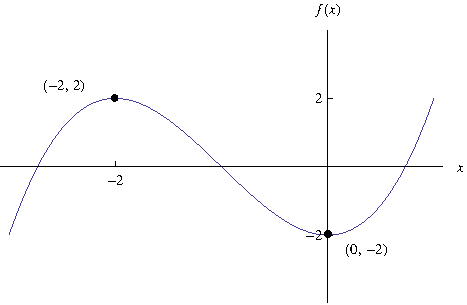
\includegraphics[width= 0.7 \textwidth,height=0.3
\textheight]{unidad2graf1.pdf}
\end{center}
\caption{$f(x) = x^{3}+3x^{2}-2$}\label{Figura15}
\end{figure}

\begin{ejemplo}
Encontar los valores m\'aximo y m\'{\i}nimo absolutos de $f(x) =
2x^{3}+3x^{2}-12x-7$ en $[-3,3]$.


\textbf{Soluci\'on:}
\medskip

\begin{enumerate}
  \item[] \textbf{1er paso.} Calculemos $\frac{df}{dx}(x)$.

\[
  \frac{df}{dx}(x)=6x^{2}+6x-12
\]

  \item[]\textbf{2o. paso.}   Determinemos los valores de $x$ en que $\frac{df}{dx} (x) = 0 $
 \begin{align*}
    \frac{df}{dx} &= 0 \\
     6x^{2}+6x-12 & = 0 \\
     x^{2}+x-2 & =0 \\
     (x+2)(x-1) &= 0
 \end{align*}
 Resolviendo las ecuaciones $x + 2 = 0$ y $x -1 = 0$, tenemos que los valores cr\'{\i}ticos son  $x_1 =
 -2$ y $x_2 = 1$.

  \item[]\textbf{3er. paso.} Hallemos la segunda derivada
\[
  \frac{d^2f}{dx^2}(x)=12x+6
\]

 \item[] \textbf{4o. paso.}
  Evaluemos  $\frac{d^2 f}{dx^{2}} (x)$ en cada  valor cr\'{\i}tico.
  Entonces
\begin{align*}
\frac{d^2 f}{dx^{2}} (-2) &= 12(-2) + 6 \\
\frac{d^2 f}{dx^{2}} (-2) &= -18
\end{align*}
Por lo que $x_1 =-2$ es la abscisa de un m\'aximo.
\begin{align*}
\frac{d^2 f}{dx^{2}} (1) &= 12(1) + 6 \\
\frac{d^2 f}{dx^{2}} (1) &= 18
\end{align*}
En consecuencia el punto $x_2 = -2$ es la abscisa de un m\'{\i}nimo.
\end{enumerate}

En conclusi\'on para encontrar los valores que corresponden al
m\'aximo y al m\'{\i}nimo se deben realizar varias sustituciones en
la funci\'on original:
\begin{align*}
 f(x) &= 2x^{3}+3x^{2}-12x-7 \\
\text{Para $x_1=-2$ se tiene} \\
 f(-2) &= 2(-2)^3 + 3(-2)^2 -12(-2) - 7 \\
 f(-2) &= 13 \\
\text{Para $x_2=1$ se tiene}\\
 f(1) &= 2 + 3 -12 - 7 \\
 f(1) &= -14
\end{align*}
Por lo que el m\'aximo relativo es el punto(-2,13) y  el m\'{\i}nimo
relativo es el punto (1,-14). Como referencia, se traza la gr�fica
de $f$ en la figura 16.
\end{ejemplo}


\begin{figure}[h]
\begin{center}
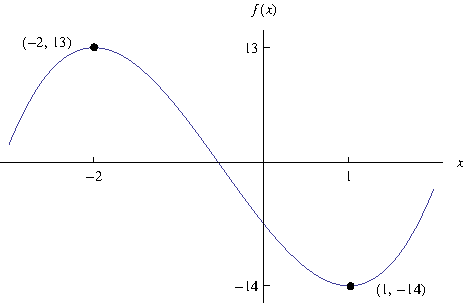
\includegraphics[width= 0.7 \textwidth,height=0.3
\textheight]{unid1graf20.pdf}
\end{center}
\caption{$f(x) = 2x^{3}+3x^{2}-12x-7$}\label{Figura15}
\end{figure}

\newpage

\begin{problema}
Un monopolista tiene una funci�n de demanda inversa $p(q) = 100-q$.
La funci�n de costo total es $C=25q$.

\begin{enumerate}
  \item \textquestiondown Cu�l es la cantidad y el precio que maximiza la utilidad?
  \item Hallar el ingreso y el costo marginal.
  \item Gr�ficar conjuntamente las funciones del ingreso, utilidad y costo.
  \item Gr�ficar conjuntamente las funciones del precio, ingreso
  marginal y costo marginal.
\end{enumerate}
\end{problema}

\textbf{Soluci\'on al problema 8}.
\begin{enumerate}
 \item La funci\'on del ingreso del monopolista es
\begin{align*}
  R(q)& =p \cdot q\\
      & =(100-q)q\\
      & =100q-q^{2}
\end{align*}
La funci�n de utilidad es
\begin{align*}
  \pi(q)& =R(q)-C(q) \\
  & =100q-q^{2}-25q \\
  & =75q-q^{2}
\end{align*}

Derivando la funci�n de utilidad obtenemos
\begin{align*}
  \pi'(q)& = 75-2q \\
  \pi'(q)& = 0 \\
       q & = 37.5
\end{align*}

Para probar que este punto es un m�ximo, obtenemos la segunda
derivada de la funci�n de la utilidad.
\[
  \pi''(q)  = -2 < 0
\]

De acuerdo con el criterio de la segunda derivada este punto es un
m�ximo. Para determinar el precio y la utilidad hacemos:
\begin{align*}
  p(q) & = 100-37.5 = \$62.50 \\
\pi(q) & = 75(37.5)-(37.5)^{2}=\$1,406.25
\end{align*}

 \item El ingreso y costo marginal son respectivamente
\begin{align*}
  R'(q) & = 100-2q \\
  C'(q) & = 25
\end{align*}

Si igualamos el ingreso marginal al costo marginal obtenemos la
cantidad que maximiza la utilidad
\begin{align*}
  R'(q) & = C'(q) \\
  100-2q & = 25 \\
  75 & = 2q \\
  q & = 37.5
\end{align*}

\newpage

\item Gr�fica del ingreso, utilidad y costo.

\begin{figure}[h]
\begin{center}
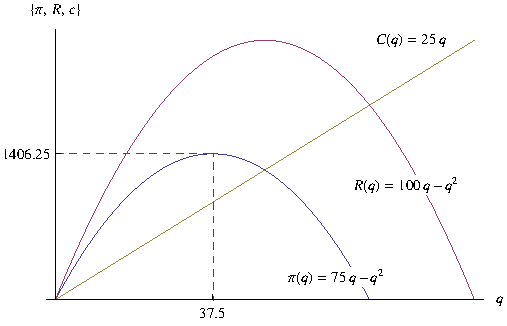
\includegraphics[width= 0.7 \textwidth,height=0.29
\textheight]{unid1graf21.pdf}
\end{center}
\caption{$R(q),\pi(q),C(q)$}\label{Figura16}
\end{figure}

\item Gr�fica del precio, ingreso marginal y costo marginal.
\begin{figure}[h]
\begin{center}
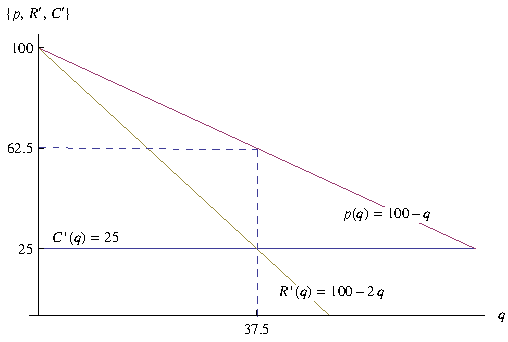
\includegraphics[width= 0.7 \textwidth,height=0.29
\textheight]{unid1graf22.pdf}
\end{center}
\caption{$p(q),C'(q),R'(q)$}\label{Figura17}
\end{figure}
\end{enumerate}

\begin{problema}
La empresa de cablevisi\'on tiene actualmente $100,000$ suscriptores
que pagan una couta mensual de  \$40 pesos. Una encuesta revel\'o
que se tendr\'{\i}an $1000$ suscriptores m\'as por cada \$0.25 de
disminuci\'on en la cuota. \textquestiondown Para qu\'e cuota se
obtendr\'a el ingreso m\'aximo y cu\'antos suscriptores se
tendr\'{\i}an entonces?
\end{problema}

\textbf{Soluci\'on del problema 9.} Sea $x$ el n\'umero de
disminuciones de \$0.25. La couta mensual es entonces de 40 - 0.25x,
donde $0 \leq x \leq 160$ y el n\'umero de suscriptores nuevos es $
1000 x$. Por lo tanto, el n\'umero total de suscriptores es $100,000
+ 1000x$. Entonces queremos maximizar el ingreso, el cu\'al esta
dado por:
\begin{align*}
  r &= (\text{n\'umero de suscriptores}) (\text{couta por suscriptor}) \\
    &= (100,000 + 1000x)(40 - 0.25x) \\
    &= 1000(100 + x)(40 - 0.25x) \\
    &= 1000(4000 + 15x - 0.25x^{2}).
\end{align*}
Haciendo $\frac{dr}{dx} = 0$ y despejamos a $x$, tenemos que:
\begin{align*}
  \frac{dr}{dx} = 1000(15 - 0.5x) & = 0 \\
                                 & =30.
\end{align*}
Como el dominio de $r$ es el intervalo cerrado $[0, 160]$, el valor
m\'aximo absoluto de $r$ debe ocurrir en $x = 30$ o en los puntos
extremos del intervalo. Ahora calculamos $r$ en estos tres puntos:
\begin{enumerate}
   \item Si $x =0$, entonces $r = 4,000,000;$
   \item Si $x = 30$, entonces $r = 4,225,000;$
   \item Si $x = 160$, entonces $r = 0$.
\end{enumerate}
De esto se sigue que el ingreso m\'aximo ocurre cuando $x = 30$.
Esto co\-rres\-pon\-de a 30 disminuciones de \$0.25, para una
disminuci\'on total de \$7.5; esto es la couta mensual \$32.50. El
n\'umero de suscriptores con esa couta son 100,000 + 30(1000) =
130,000.

\newpage

\begin{problema}
Una empresa tiene una funci\'on dada por $ q (L) = aL-bL ^ 2 $, donde $L$ es el n\'umero de trabajadores empleados por la empresa y $ a, b> 0 $. El producto de la empresa se vende a un precio de $p$, y el salario promedio de un trabajador es $w$. Encontrar el n\'umero de trabajadores que maximiza el beneficio de la empresa. Demostrar que el beneficio es, en efecto, un m\'aximo.
\medskip

\textbf{Soluci\'on al Problema 10.}
\medskip

Expresamos la ganancia como la diferencia entre los ingresos totales y el costo total
\begin{align*}
    \pi(L) &=  p(aL - bL^2) - wL \\
    \pi'(L) &=  ap - 2bpL - w = 0  \qquad \pi''(L)= - 2bp< 0  \ \text{implica un m\'aximo} \\
    L^{*} &= \frac{ap- w}{2bp}
\end{align*}

Por lo tanto, el n\'umero \'optimo de trabajadores y el salario promedio se ven relacionados, como dicta la l\'ogica econ\'omica.
\end{problema}

\medskip

\begin{problema} Una empresa tiene una funci\'on de producci�n Cobb-Douglas $ q = 10 K ^ {\frac{3}{5}} L ^ {\frac{2}{5}}$, y vende sus productos a un precio de 30. La empresa opera en el corto plazo con un n\'umero fijo  de m\'aquinas en 32. Buscar el m\'aximo beneficio de la empresa, si se sabe que el precio de una m\'aquina es de 120 y el salario de los trabajadores es de 15 unidades.
\medskip

\textbf{Soluci\'on al Problema 11.}
    Restando el costo total de capital y el trabajo de los ingresos totales da la ecuaci\'on de beneficios:
    \begin{align*}
    \pi &= pq - rK - wL = 30 (10)32^{\frac{3}{5}}L^{\frac{2}{5}} - 120(32) - 15L \\
    \pi(L) &= 300(32)^{\frac{3}{5}}L^{\frac{2}{5}} - 120 (32) - 15(L) = 300(8)L^{\frac{2}{5}}-
    3840- 15L \\
    &= 2400 L^{\frac{2}{5}}- 3840 - 15L
    \end{align*}
    La maximizaci\'on de beneficios con respecto a la mano de obra
    \begin{align*}
    \pi'(L) &=  \frac{2400 (2)}{5} L^{-\frac{3}{5}} - 15 = 0 \quad \pi''(L)= -576L^{-\frac{8}{5}}< 0  \\
    960L^{-\frac{3}{5}} &=  15 \\
    L^{\frac{3}{5}} &= 64 \\
    L &= 64^{\frac{5}{3}} \\
    L^{*} &= 1024  \ \text{ trabajadores} \\
    \pi(1024) &= 2400(1024)^{\frac{2}{5}} - 3840 - 15 (1024)\\
    & = 2400(16)- 3840-15360\\
    & = 19,200
    \end{align*}
\end{problema}

\newpage

\setcounter{page}{1}

\begin{center}
\textbf{TAREA 1: M�XIMOS Y M�NIMOS}
\end{center}

Trabajo individual.
\medskip


En los ejercicios 1 al 8, encontrar los valores m\'aximos,
m\'{\i}nimos absolutos de cada funci\'on en el intervalo dado.
Despu�s graficar la funci�n en la computadora,  comprobando los
puntos en donde se alcanzan los extremos absolutos.
\begin{align*}
1. \,  f(x) &= \frac{x^3}{3}  - \frac{x^2}{2}  - 2x + \frac{1}{3} &
& -3 \leq x \leq 4 \\[.3cm]
2. \,  f(x) & = \frac{x^4}{4}  -2x^2 + 4                           &
&-3 \leq x \leq 3  \\[.3cm]
3. \,  f(x) & = x^3 -3x + 3     & &-3\leq x \leq 3   \\[.3cm]
4. \,  f(x) & =-2x^3  + 6x^2 - 3                           & &-1
\leq x \leq 3  \\[.3cm]
5. \,  f(x) & =x^2-\frac{x^4}{8}                            & &-3
\leq x \leq 3  \\[.3cm]
6. \,  f(x) & = 2x^3  + 3x^2 -12x -7                           & &-4
\leq x \leq 3 \\[.3cm]
7. \,  f(x) & = x^2 - 8 \ln x                            & & 0 
< x \leq 4  \\[.3cm]
8. \,  f(x) & = \frac{1}{\sqrt{2 \pi}} e^{ - \frac{x^2}{2}} & & -5
\leq x \leq 5
\end{align*}

\newpage

\setcounter{page}{1}

\begin{center}
\textbf{TAREA 2: M�XIMOS Y M�NIMOS APLICADOS A LA ECONOM�A}
\end{center}

Trabajo en equipo con dos o tres integrantes.
\medskip

\hspace{.2cm} \textbf{Teor\'{\i}a Microecon\'omica: problemas de
maximizaci\'on del be\-ne\-fi\-cio}

\vspace{.3cm}

En los problemas  del 1 al 6, $C(q)$ es el costo total de producir
$q$ unidades de un bien y $p(q)$ es el precio al cual se vender\'an
las $q$ unidades.

\begin{enumerate}
 \item[a)] \textquestiondown Cu�l es la cantidad y el precio que maximiza la utilidad?. \vspace{.2cm}
 \item[b)] Hallar el ingreso y el costo marginal. \vspace{.2cm}
 \item[c)] Utilizar Excel o el software de su preferencia para calcular
  los valores del ingreso, beneficio, costo, precio, ingreso
  marginal y costo marginal en el rango solicitado. \vspace{.2cm}
 \item[d)] Graficar conjuntamente las funciones del ingreso, beneficio y
 costo. \vspace{.2cm}
 \item[e)] Graficar conjuntamente las funci\'on del precio, ingreso marginal y
 costo marginal. \vspace{.2cm}
\end{enumerate}

\begin{enumerate}
 \item $p(q) = 75-3q \quad ; \quad C(q) = \frac{1}{5}q^2 + 4 q + 27 \quad 0 \leq q \leq 15$
 \item $p(q) = 45-4q \quad ; \quad C(q) = \frac{1}{4}q^2 + 3 q + 7
 \quad 0 \leq q \leq 10$
 \item $p(q) = 100-q \quad ; \quad C(q) = 25q \quad 0 \leq q \leq 60$
 \item $p(q) = 50-2q \quad ; \quad C(q) = 20 + 2q + \frac{1}{2}q^2
 \quad 0 \leq q \leq 15$
 \item $p(q) = 150-2q \quad ; \quad C(q) = \frac{1}{10} q^3 - 3q^2 + 50 q + 100
 \quad 0 \leq q \leq 35$
 \item $p(q) = 200-2q \quad ; \quad C(q) = \frac{2}{3}q^3 - 14q^2 +
 222q+50 \quad 0 \leq q \leq 18$
\end{enumerate}

\vspace{.2cm}

\newpage

\textbf{Teor\'{\i}a Macroecon\'omica: Modelo de demanda de trabajo.}

\vspace{.2cm}

Suponga que para producir el bien $q$ solo se emplea el capital
$(K)$ y el trabajo $(L)$. El trabajo puede variar libremente
mientras que el capital es fijo. As\'{\i} que la funci\'on de
producci\'on toma la forma
\begin{equation*}
 q = q(L,\bar{K})
\end{equation*}
El objetivo del empresario racional es maximizar el beneficio, la
diferencia entre ingresos, $Y$ y costos totales, $CT$.

\begin{equation*}
  \pi = Y - CT
\end{equation*}

donde el ingreso esta determinado por:

\begin{equation*}
   Y = pq
\end{equation*}

y la funci\'on de costos totales es:
\begin{equation*}
  CT = \overline{CF} +  CV + \overline{CF} +WL
\end{equation*}
donde $W$ es el salario o precio del trabajo y $CF$ son los costos
fijos generados por el uso del capital.

\begin{enumerate}
  \item[a)] Demostrar que la funci\'on de beneficios es:
  \[
      \pi = q(L,\bar{K})p- \overline{CF} -WL
  \]
  \item[b)] Obtener la demanda \'optima de trabajo e interpretar su
  resultado.
\end{enumerate}

\end{document}
